\documentclass[10pt,landscape]{article}
\usepackage{multicol}
\usepackage{calc}
\usepackage{ifthen}
\usepackage[landscape]{geometry}
\usepackage{graphicx}
\usepackage{amsmath, amssymb, amsthm}
\usepackage{latexsym, marvosym}
\usepackage{pifont}
\usepackage{lscape}
\usepackage{graphicx}
\usepackage{array}
\usepackage{booktabs}
\usepackage[bottom]{footmisc}
\usepackage{tikz}
\usepackage{breqn}
\usetikzlibrary{shapes}
\usepackage{pdfpages}
\usepackage{wrapfig}
\usepackage{amssymb, amsmath, amsthm}
\usepackage{mathtools}
\usepackage{tabularx}
\usepackage{enumitem}
\setlist[description]{leftmargin=0pt}
\usepackage{xfrac}
\usepackage[
            open,
            openlevel=2
            ]{bookmark}
\usepackage{relsize}
\usepackage{rotating}

 \newcommand\independent{\protect\mathpalette{\protect\independenT}{\perp}}
    \def\independenT#1#2{\mathrel{\setbox0\hbox{$#1#2$}%
    \copy0\kern-\wd0\mkern4mu\box0}} 
            
\newcommand{\noin}{\noindent}    
\newcommand{\logit}{\textrm{logit}} 
\newcommand{\var}{\textrm{Var}}
\newcommand{\cov}{\textrm{Cov}} 
\newcommand{\corr}{\textrm{Corr}} 
\newcommand{\N}{\mathcal{N}}
\newcommand{\Bern}{\textrm{Bern}}
\newcommand{\Bin}{\textrm{Bin}}
\newcommand{\Beta}{\textrm{Beta}}
\newcommand{\Gam}{\textrm{Gamma}}
\newcommand{\Expo}{\textrm{Expo}}
\newcommand{\Pois}{\textrm{Pois}}
\newcommand{\Unif}{\textrm{Unif}}
\newcommand{\Geo}{\textrm{Geo}}
\newcommand{\NBin}{\textrm{NBin}}
\newcommand{\Hypergeometric}{\textrm{HGeom}}
\newcommand{\HGeom}{\textrm{HGeom}}
\newcommand{\Mult}{\textrm{Mult}}

\DeclareMathOperator{\sinc}{sinc}


\geometry{top=.4in,left=.2in,right=.2in,bottom=.4in}

\pagestyle{empty}
\makeatletter
\renewcommand{\section}{\@startsection{section}{1}{0mm}%
                                {-1ex plus -.5ex minus -.2ex}%
                                {0.5ex plus .2ex}%x
                                {\normalfont\large\bfseries}}
\renewcommand{\subsection}{\@startsection{subsection}{2}{0mm}%
                                {-1explus -.5ex minus -.2ex}%
                                {0.5ex plus .2ex}%
                                {\normalfont\normalsize\bfseries}}
\renewcommand{\subsubsection}{\@startsection{subsubsection}{3}{0mm}%
                                {-1ex plus -.5ex minus -.2ex}%
                                {1ex plus .2ex}%
                                {\normalfont\small\bfseries}}
\makeatother

\setcounter{secnumdepth}{0}

\setlength{\parindent}{0pt}
\setlength{\parskip}{0pt plus 0.5ex}

% -----------------------------------------------------------------------

\usepackage{titlesec}

\titleformat{\section}
{\color{blue}\normalfont\large\bfseries}
{\color{blue}\thesection}{1em}{}
\titleformat{\subsection}
{\color{cyan}\normalfont\normalsize\bfseries}
{\color{cyan}\thesection}{1em}{}
% Comment out the above 5 lines for black and white

\begin{document}

\raggedright
\footnotesize
\begin{multicols*}{3}

% multicol parameters
% These lengths are set only within the two main columns
%\setlength{\columnseprule}{0.25pt}
\setlength{\premulticols}{1pt}
\setlength{\postmulticols}{1pt}
\setlength{\multicolsep}{1pt}
\setlength{\columnsep}{2pt}

%%%%%%%%%%%%%%%%%%%%%%%%%%%%%%%%%%%%
%%% TITLE
%%%%%%%%%%%%%%%%%%%%%%%%%%%%%%%%%%%%

\begin{center}
    {\color{blue} \Large{\textbf{Probability Cheatsheet}}} \\
   % {\Large{\textbf{Probability Cheatsheet}}} \\
    % comment out line with \color{blue} and uncomment above line for b&w
\end{center}

%%%%%%%%%%%%%%%%%%%%%%%%%%%%%%%%%%%%
%%% ATTRIBUTIONS
%%%%%%%%%%%%%%%%%%%%%%%%%%%%%%%%%%%%

\scriptsize

Compiled by Eigen-$\pi$ (\url{https://www.linkedin.com/in/islamibr29/}).  Licensed under \texttt{\href{http://creativecommons.org/licenses/by-nc-sa/4.0/}{CC BY-NC-SA 4.0}}. Please share comments, suggestions, and errors at \url{http://github.com/islamibr/today_i_learned}.

\begin{center}
    Last Updated \today
\end{center}

%%%%%%%%%%%%%%%%%%%%%%%%%%%%%%%%%%%%
%%% BEGIN CHEATSHEET
%%%%%%%%%%%%%%%%%%%%%%%%%%%%%%%%%%%%

\section{Prerequisites}
\begin{itemize}
    \item Binomial Expansion $$
\begin{aligned}
& \sum_{n=0}^{\infty} a^n = 1+a+a^2+a^3+\cdots=\frac{1}{1-a} \\
& \sum_{n=1}^{\infty} a^n = a(1+a+a^2+a^3+a^4+\cdots)=\frac{a}{1-a} \\
& \sum_{n=0}^{\infty} (n+1)a^n = 1+2 a+3 a^2+4 a^3+\cdots=\frac{1}{(1-a)^2}
\end{aligned}
$$
    \item Taylor Expansion$$
\begin{aligned}
& (1+x)^k = \sum_{n=0}^{\infty} \binom{k}{n} x^n \\
& e^x=\sum_{n=0}^{\infty} \frac{x^n}{n !} \\
& \sin x=\sum_{n=0}^{\infty}(-1)^n \frac{x^{2 n+1}}{(2 n+1) !} \\ & \cos x=\sum_{n=0}^{\infty}(-1)^n \frac{x^{2 n}}{(2 n) !} \\
\end{aligned}
$$
    
\item Trig Identities \[
\begin{aligned}
    & \sin (\alpha+\beta)=\sin \alpha \cos \beta+\cos \alpha \sin \beta \\
    & \cos (\alpha+\beta)=\cos \alpha \cos \beta-\sin \alpha \sin \beta \\
    & \sin (\alpha-\beta)=\sin \alpha \cos \beta-\cos \alpha \sin \beta \\
    & \cos (\alpha-\beta)=\cos \alpha \cos \beta+\sin \alpha \sin \beta \\ \\
    &  \sin \alpha \cos \beta= \frac{1}{2} [\sin (\alpha+\beta)+\sin (\alpha-\beta)] \\
    & \cos \alpha \sin \beta=\frac{1}{2} [\sin (\alpha+\beta)-\sin (\alpha-\beta)] \\
    & \cos \alpha \cos \beta=\frac{1}{2} [\cos (\alpha+\beta)+\cos (\alpha-\beta)] \\
    & \sin \alpha \sin \beta=\frac{1}{2} [\cos (\alpha-\beta)-\cos (\alpha+\beta)] \\ \\
    & \cos(\alpha + \pi) = -\cos(\alpha) \\ & \cos(\alpha + 2\pi) = \cos(\alpha) \\
\end{aligned}
\]

\item Fourier Transform
\begin{center}
    \begin{tabular}{c|c}
$g(t)$ & $G(f)$  \\ \hline
$A \operatorname{rect}\left(\frac{t}{T}\right)$ & $A T \sinc (f T)$ \\ \hline
$\mathrm{e}^{-\mathrm{at}} \mathrm{u}(\mathrm{t}), \mathrm{a}>0$ & $\frac{1}{a+j 2 \pi f}$ \\ \hline
$\mathrm{e}^{-\mathrm{a} \mid \mathrm{t} \mid}, \mathrm{a}>0$ & $\frac{2 a}{a^2+(2 \pi f)^2}$ \\ \hline
$\mathrm{e}^{-\pi \mathrm{t}^2}$ & $e^{-\pi f^2}$ \\ \hline
$\delta(t)$ & 1 \\ \hline
1 & $\delta(\mathrm{f})$ \\ \hline
$\delta\left(t-t_0\right)$ & $e^{-j 2 \pi t_0 f}$ \\ \hline
$e^{j 2 \pi f_c t}$ & $\delta\left(f-f_c\right)$ \\ \hline
$\cos \left(2 \pi f_c t\right)$ & {$\left[\delta\left(f-f_c\right)+\delta\left(f+f_c\right)\right] / 2$} \\ \hline
$\sin \left(2 \pi f_c t\right)$ & {$\left[\delta\left(f-f_c\right)-\delta\left(f+f_c\right)\right] / 2 j$} \\
\end{tabular}
\end{center}

\end{itemize}



\section{Axioms of Probability}
\begin{itemize}
    \item  Non negativity : ensures that probability is never negative.
$$
\mathbb{P}[A] \geq 0
$$
\item Normalization : ensures that probability is never greater than 1.
$$
\mathbb{P}[\Omega]=1
$$

\item Additivity : allows us to add probabilities when two events do not overlap.
$$
\mathbb{P}\left[\bigcup_{i=1}^{\infty} A_i\right]=\sum_{i=1}^{\infty} \mathbb{P}\left[A_i\right]
$$



\end{itemize}


\section{Contional probability}



$$ \mathbb{P}[A|B] = \frac{\mathbb{P}[A\cap B]}{\mathbb{P}[B]}  $$

\begin{itemize}
\item Independence : Two events A and B are independent if :
\begin{align*}
 \mathbb{P}[A|B] &=  \mathbb{P}[A] \\
\text{or} \qquad \mathbb{P}[A\cap B] &=  \mathbb{P}[A]\mathbb{P}[B]  
\end{align*}
\item Note:
$$\text{Disjoint}  \nLeftrightarrow \text{Independent}$$

\item {Unions of Two Non-Disjoint Sets}
$$ \mathbb{P}[A\cup B] = \mathbb{P}[A] + \mathbb{P}[B] - \mathbb{P}[A\cap B] $$
\item {Unions of Two Non-Disjoint Sets in Independent case}
$$ \mathbb{P}[A\cup B] = 1 - \mathbb{P}[A^c\cap B^c] $$

If A and B are disjoint, then $A \cap B = \phi$. This only implies that $\mathbb{P}[ A \cap B] = 0$.

\item Law of Total Probability :

$$ \mathbb{P}[A] = \sum_{i=1}^n \mathbb{P}[A|B_i] \mathbb{P}[B_i] $$

\item Bayes' rule 
$$ \mathbb{P}[A|B] = \frac{\mathbb{P}[B|A]\mathbb{P}[A]}{\mathbb{P}[B]}  $$

\end{itemize}

\section{Series and Parallel Circuits}

\begin{itemize}


\item Series devices:
\begin{dgroup*}
  \begin{dmath*}
$$\mathbb{P}[\text{Circuit \textbf{operates}}] = \mathbb{P}[\text{device 1 \textbf{operates}}] \times \mathbb{P}[\text{device 2 \textbf{operates}}] \times \cdots \times \mathbb{P}[\text{device n \textbf{operates}}] $$
  \end{dmath*}
\end{dgroup*}

\item Parallel devices:
\begin{dgroup*}
  \begin{dmath*}
$$\mathbb{P}[\text{Circuit \textbf{fails}}] = \mathbb{P}[\text{device 1 \textbf{fails}}] \times \mathbb{P}[\text{device 2 \textbf{fails}}] \times \cdots  \mathbb{P}[\text{device n \textbf{fails}}] $$
  \end{dmath*}
\end{dgroup*}
\item Remember :  $$\mathbb{P}[\text{failure}] = 1 - \mathbb{P}[\text{success}]$$
\end{itemize}


\section{Techniques of Counting}
\begin{itemize}
\item Arranging $n$ items in $n$ places : number of ways $$n!$$
\item Permutations : 
$$ \Myperm{k} = \frac{n!}{(n-k)!} $$

\item Combinations : 
$$ \Mycomb{k} = \frac{n!}{k!(n-k)!} $$
\end{itemize}
\setlength{\extrarowheight}{10pt}


\begin{center}
  \begin{tabular}{|l||c|c|}
    \hline
    & order & no order \\
    \hline \hline
    replacement & $n^r$ & ${}^{n-r+1} C_r$ \\
    \hline
    no replacement & ${}^n P_r$ & ${}^n C_r$ \\
    \hline
\end{tabular}  
\end{center}


%\begin{tabu} to \textwidth {@{} l *5{X[c]}@{}}
%1 & 2 & 3 & 4 & 5 & 6\\
%\end{tabu}

\section{Discrete Random Variables}
\begin{itemize}
\item What are random variables?\\
Random variables are mappings from events to numbers.
\item  probability mass function (PMF) of a random variable $X$ is a function which specifies the probability of obtaining a number $x$. 
$$p_X(x) = \mathbb{P}[X=x]$$
\item Note that a PMF should satisfy the following condition 
$$\sum_{x\in X(\Omega)} p_X(x) = 1 $$

\item Cumulative distribution function CDF  :
$$ F_X(x_k) = \pp[X \leq x_k] = \sum_{l=-\infty}^k p_X(l) $$


\item What is expectation?\\
Expectation = Mean = Average computed from a PMF.
$$ \mathbb{E}[X] = \mu = \sum_{x \in X(\Omega)}xp_X(x) $$

\item Properties:
$$ \mathbb{E}[g(X)] = \sum_{x \in X(\Omega)}g(X) p_X(x) $$

$$\mathbb{E}[aX+b] =a\mathbb{E}[X]+b $$

\item What is variance?\\
It is a measure of the deviation of the random variable X relative to its mean.
\begin{align*}
\text{Var}[X] = \sigma^2 &= \mathbb{E}[(X- \mu)^2] \\
&=\mathbb{E}[X^2]  - \mathbb{E}[X]^2\\
&=\mathbb{E}[X^2]  - \mu^2
\end{align*}
\item Properties:

$$\text{Var}[aX+b] =a^2 \text{Var}[X] $$
\item Coefficient of variance = $\dfrac{\sigma}{\mu}$
\end{itemize}
\section{Special Discrete Random Variables}
\subsection{Bernoulli} (a coin-flip random variable)
\begin{itemize}
\item $\pp[\text{sucess}] = p,\; \pp[\text{failure}] = 1-p = q$
\item PMF :
$$ p_X(0) = 1-p \qquad p_X(1) = p$$
\item Expectation:
$$ \mathbb{E}[X] = p $$

\item Variance:
\begin{align*}
\text{Var}[X] &= p(1-p) \\
&= pq
\end{align*}
\end{itemize}
\subsection{Bionomial} ($n$ times coin-flips random variable)
\begin{itemize}


\item $\pp[\text{sucess}] = p,\; \pp[\text{failure}] = 1-p = q$
\item PMF :
$$ p_X(k) = \Mycomb{k} p^k q^{n-k}$$
\item Expectation:
$$ \mathbb{E}[X] = np $$

\item Variance:
\begin{align*}
\text{Var}[X] &= np(1-p) \\
&= npq
\end{align*}
\item Show that the binomial PMF sums to 1.:\\
Use the binomial theorem:
\begin{align*}
\sum_{k=0}^n p_X(k) &= \sum_{k=0}^n \Mycomb{k} p^k q^{n-k}\\ &= (p+(1-p))^n\\ &=1 
\end{align*}

\end{itemize}

\subsection{Geometric} (Trying a binary experiment until we succeed random variable)
\begin{itemize}


\item $\pp[\text{sucess}] = p,\; \pp[\text{failure}] = 1-p = q$
\item PMF :
$$ p_X(k) = \underbrace{(1-p)^{k-1}}_{k-1 \ \text{failures}}\underbrace{p}_{\text{final success}}$$
\item CDF: $$1-q^x$$
\item Expectation:
$$ \mathbb{E}[X] = \frac{1}{p} $$

\item Variance:
\begin{align*}
\text{Var}[X] &= \frac{1-p}{p^2} \\
&= \frac{q}{p^2}
\end{align*}

\end{itemize}

\subsection{Poisson} (For small p and large n where $\lambda$ = $np$)
\begin{itemize}


\item $\lambda$ = the rate of the arrival
\item PMF :
$$ p_X(k) = e^{-\lambda} \frac{\lambda^k}{k!}$$
\item Expectation:
$$ \mathbb{E}[X] = \lambda $$

\item Variance:
\begin{align*}
\text{Var}[X] = \lambda 
\end{align*}

\item Show that the Poisson PMF sums to 1.:\\
Use the exponential series:
\begin{align*}
\sum_{k=0}^\infty p_X(k) &= \sum_{k=0}^\infty e^{-\lambda} \frac{\lambda^k}{k!}\\ &= e^{-\lambda} \underbrace{\sum_{k=0}^\infty \frac{\lambda^k}{k!}}_{=e^{\lambda}}\\ &=1 
\end{align*}

\end{itemize}

\section{Continuous Random Variables}
\begin{itemize}

\item  probability density function (PDF) is a continuous version of a PMF, we integrate PDF to compute the probability
$$ \pp[a\leq X \leq b] = \int_a^b f_X(x) \, dx $$



\item Note that a PMF should satisfy the following condition 
$$\int_{\Omega} f_X(x)\, dx = 1 $$

\item Note : 
$$\pp[X=\text{certian point} ] = 0 $$

\item Cumulative distribution function CDF  :
$$ F_X(x_k) = \pp[X \leq x] = \int_{-\infty}^x f_X(t) dt $$

\item Note:
\begin{align*}
\text{CDF} &= \int \text{PDF}\\
\text{PDF} &= \frac{d}{dx} \text{PDF}
\end{align*}


\item Expectation (Mean):
$$ \mathbb{E}[X] = \mu =\int_{\Omega} x\,f_X(x) dx  $$

\item Properties:
$$ \mathbb{E}[g(X)] = \mu =\int_{\Omega} g(X)\,f_X(x) dx  $$


$$\mathbb{E}[aX+b] =a\mathbb{E}[X]+b $$

\item Mode: the peak of the PDF

How to find the mode from PDF:
\begin{itemize}
    \item Find a point \(c\) such that \(f_X(c)\) is maximized by differentiation (and test the edges of the interval).
\end{itemize}

How to find the mode from CDF:
\begin{itemize}
    \item Continuous: Find a point \(c\) such that \(F_X(c)\) has the steepest slope.
    \item Discrete: Find a point \(c\) such that \(F_X(c)\) has the biggest gap in a jump.
\end{itemize}


\item Median: (a point c that separates the PDF into two equal areas)
$$\pp[x<c] = \pp[x>c] = 0.5$$
$$F_X(c) = 0.5$$

\item Note : Symmetric distribution is a distribution in which Median = Mean

\item Percentiles: \\ 
To get the $\alpha$ percentile, find the value $c$ at which $$F_X(c) = \alpha$$

\item Variance:
\begin{align*}
\text{Var}[X] = \sigma^2 &= \mathbb{E}[(X- \mu)^2] \\
&=\int_{\Omega} (x-\mu)^2f_X(x) dx \\
&=\mathbb{E}[X^2]  - \mathbb{E}[X]^2\\
&=\mathbb{E}[X^2]  - \mu^2
\end{align*}
\item Properties:

$$\text{Var}[aX+b] =a^2 \text{Var}[X] $$

\end{itemize}

\section{Special Continuous Random Variables}
\subsection{Uniform} 
\begin{itemize}

\item PDF :
$$ f_X(x) =
\begin{dcases}
\frac{1}{b-a} & a \leq x \leq b\\
0 & \text{otherwise}\\
\end{dcases}
$$
\item CDF :
$$F\frac{x-a}{b-a}$$

\item Expectation:
$$ \mathbb{E}[X] = \frac{a+b}{2} $$

\item Variance:
\begin{align*}
\text{Var}[X] = \frac{(a-b)^2}{12}
\end{align*}
\end{itemize}

\subsection{Exponential} 
\begin{itemize}

\item What is the origin of exponential random variables?
\begin{itemize}
\item An exponential random variable is the \emph{interarrival} time between two consecutive
Poisson events.

\end{itemize}

\item PDF :
$$ f_X(x) =
\begin{dcases}
\lambda e ^{-\lambda x} & x \geq 0\\
0 & \text{otherwise}\\
\end{dcases}
$$



\item CDF :
$$ F_X(x) =
\begin{dcases}
0 & x < 0\\
1- e^{-\lambda x} & x \geq 0\\
\end{dcases}
$$



\item Expectation:
$$ \mathbb{E}[X] = \frac{1}{\lambda} $$

\item Variance:
\begin{align*}
\text{Var}[X] = \frac{1}{\lambda^2}
\end{align*}

\item Memorylessness property:
\begin{align*}
\pp[T< t+m | T>t] = \pp[T<m] = F_X(m)
\end{align*}

\item Starting from poisson distribution, derive an expression of PDF of exponential random variable

\begin{align*}
&\text{We assume that N is Poisson with a parameter }\lambda t \, \\ & \text{or any duration }t : \\
&\pp[N=n]=e^{-\lambda t} \frac{(\lambda t) ^n}{n!}\\
&\text{Let $T$ be the interarrival time between two events}\\
&\pp[T>t] = \pp[\text{interarrival time}>t] = \pp[\text{no arrival in t}]\\& = \pp[N=0]=e^{-\lambda t} \frac{(\lambda t) ^0}{0!} = e^{- \lambda t}
\end{align*}

\begin{align*}
&\text{since}, \,\, \pp[T>t] = 1 - F_T(t)\\
&\therefore  F_T(t) = 1 - e^{- \lambda t}\\
&f_T(t) = \frac{d}{dx} F_T(t) = \lambda e^{- \lambda t}
\end{align*}

\end{itemize}


\subsection{Erlang-k} 
(A generalization of the exponential distribution is the length until r counts occur in a Poisson process. )
\begin{itemize}



\item PDF :
$$ f_X(x) = \frac{\lambda^k e ^{-\lambda x} x ^{k-1}}{(k-1)!}
$$

\item CDF :
$$\int_{-\infty}^{X'} \frac{\lambda^k e ^{-\lambda x} x ^{k-1}}{(k-1)!} dx$$





\item Expectation:
$$ \mathbb{E}[X] = \frac{k}{\lambda} $$

\item Variance:
\begin{align*}
\text{Var}[X] = \frac{k}{\lambda^2}
\end{align*}


\end{itemize}


\subsection{Gamma} 

\begin{itemize}



\item PDF :
$$ f_X(x) = \frac{1}{\beta^r \Gamma (\alpha)} x^{\alpha - 1} e^{-x/\beta}
$$
$\alpha$ : Shape parameter\\
$\beta$ : Scale parameter\\







\item Expectation:
$$ \mathbb{E}[X] = \alpha \beta $$

\item Variance:
\begin{align*}
\text{Var}[X] =\alpha \beta^2
\end{align*}


\item Starting from gamma distribution, derive an expression of PDF for erlang-k random variable

\begin{align*}
&f_X(x) = \frac{1}{\beta^r \Gamma (\alpha)} x^{\alpha - 1} e^{-x/\beta}\\
&\text{Substitute $\alpha$ = $k$ and $\beta$ = $\frac{1}{\lambda}$ }\\
 &f_X(x) = \frac{\lambda^k e ^{-\lambda x} x ^{k-1}}{\Gamma(k)}\\
& \text{ \underline{\textbf{If k is an integer}}, X has an Erlang distribution.}\\
& f_X(x) = \frac{\lambda^k e ^{-\lambda x} x ^{k-1}}{(k-1)!}
\end{align*}

\item Exponential distribution is a special case of Gamma distribution with $\alpha = 1$ and $\beta = \dfrac{1}{\lambda}$

\item Chi-Squared distribution $\chi^2$ is a special case of Gamma distribution with $\alpha = v/2$ and $\beta =2$ \\
it is a important distribution in statistics, also called as number of degrees of freedom
\end{itemize}




\subsection{Gaussian} 
\begin{itemize}
\item We write $$X \sim \mathcal{N}(\mu,\,\sigma^{2})$$

\item PDF :
$$f_X(x) = \frac{1}{\sigma\sqrt{2\pi}} 
  \exp\left( -\frac{1}{2}\left(\frac{x-\mu}{\sigma}\right)^{\!2}\,\right)
$$


\item Expectation:
$$ \mathbb{E}[X] = \mu $$

\item Variance:
\begin{align*}
\text{Var}[X] = \sigma^2
\end{align*}
\end{itemize}

\subsection{Standard Gaussian} 
\begin{itemize}
\item We write $$Z \sim \mathcal{N}(0,\,1)$$

\item Conversion from Gaussian to Standard Gaussian 
$$ Z = \frac{X - \mu}{\sigma}$$ 

\item PDF :
$$f_Z(z) = \frac{1}{\sqrt{2\pi}} 
e^{-\dfrac{z^2}{2}}
$$

\item CDF:
\begin{align*}
&\Phi (z) = \pp[Z < z]\\
&\pp[Z > z] = 1 - \Phi (z)\\
&\Phi (-z) = 1 - \Phi (z)
\end{align*}

\item Expectation:
$$ \mathbb{E}[X] = \mu = 0 $$

\item Variance:
\begin{align*}
\text{Var}[X] = \sigma^2 = 1
\end{align*}
\end{itemize}


\section{Moment generating function}

\begin{itemize}
\item MGF:
$$ M_X(t) = \mathbb{E}[e^{tX}] $$
\item r\textsuperscript{th} moment:
$$ \mathbb{E}[X^r] = \left. \frac{d^r}{dt^r} M_X(t) \right|_{t=0} $$

\end{itemize}

\section{Joint Discrete Probability}
\begin{itemize}
\item 
$$ f_{XY}(x,\,y) = \pp[X=x,\,Y=y] $$
\item Properties :
$$ \sum_X \sum_Y f_{XY}(x,\,y) = 1 $$

\item Marginal PMF :
$$ f_X(x) = \sum_Y f_{XY}(x,\,y) $$
$$ f_Y(x) = \sum_X f_{XY}(x,\,y) $$
\item Independence : X and Y are independent if
$$ \underbrace{f_{XY}(x,y) =  f_{X}(x) \times   f_{Y}(y)} _{\text{for all values of x and y}} $$

also if :
$$ f_{X|Y} = f_X $$
$$ f_{Y|X} = f_Y $$

\item Conditional probability:

\begin{align*}
f_{Y|X} = \frac{f_{XY}(x,\,y)}{f_X(x)}\\
f_{X|Y} = \frac{f_{XY}(x,\,y)}{f_Y(y)}\\
\end{align*}
\end{itemize}




\section{Joint Continuous Probability}
\begin{itemize}
$$  \pp[\Lambda] = \iint_{\Lambda} f_{XY}\; dx\;dy $$
$$\text{for any event } \Lambda \subseteq \Omega_X \times  \Omega_Y$$
\item Properties :
$$ \iint_A f_{XY}(x,\,y)\; dA = 1 $$

\item Marginal PMF :
$$ f_X(x) = \int_Y f_{XY}(x,\,y)  \;dy$$
$$ f_Y(x) = \int_X f_{XY}(x,\,y) \;dx$$
\item Independence : X and Y are independent if
$$ {f_{XY}(x,y) =  f_{X}(x) \times   f_{Y}(y)}  $$

also if :
$$ f_{X|Y} = f_X $$
$$ f_{Y|X} = f_Y $$

\item Conditional probability:

\begin{align*}
f_{Y|X} = \frac{f_{XY}(x,\,y)}{f_X(x)}\\
f_{X|Y} = \frac{f_{XY}(x,\,y)}{f_Y(y)}\\
\end{align*}
\end{itemize}

\section{Expectation, Covariance and Correlation}
\begin{itemize}

\item Discrete:
$$ \mathbb{E}[g(x,\,y)] = \sum_X \sum_Y g(x,\,y) \, f_{XY}(x,\,y) $$


\item Continuous:
$$ \mathbb{E}[g(x,\,y)] = \int_X \int_Y g(x,\,y) \, f_{XY}(x,\,y) dx\, dy $$

\item Properties:

$$ \mathbb{E}[x+y] =  \mathbb{E}[x] + \mathbb{E}[y]$$

\item if $x$ and $y$ are independent:

$$ \mathbb{E}[xy] =  \mathbb{E}[x] \mathbb{E}[y]$$

\item Covariance:
\begin{align*}
\text{Cov}(X,\,Y) = \sigma_{XY} &= \mathbb{E}[(X-\mu_X)(Y-\mu_Y)]\\
&= \mathbb{E}[XY] - \mathbb{E}[X]\mathbb{E}[Y]
\end{align*}

\item Variance:

\begin{align*}
\mathbb{V}[X+Y] = \mathbb{V}[X]  + \mathbb{V}[Y] +2 \text{Cov}(X,\,Y)
\end{align*}

\item if $x$ and $y$ are independent:

$$ \mathbb{V}[X+Y] = \mathbb{V}[X]  + \mathbb{V}[Y] $$

\item Correlation Coefficient:

\begin{align*}
\rho_{X,Y} = \frac{\text{Cov}(X,\,Y)}{\sigma_{X}\sigma_{Y}}
\end{align*}

\end{itemize}

\section{CLT and Rayleigh Distribution}
\subsection{CLT}
$$\lim _{n \rightarrow \infty} P\left(\frac{\bar{X}-\mu}{\sigma / \sqrt{n}}<x\right)=\Phi(x)$$
$$\overline{\mathrm{X}}=\frac{1}{\mathrm{n}} \sum_{\mathrm{i}=1}^{\mathrm{n}} \mathrm{X}_{\mathrm{i}} \sim \operatorname{Normal}\left(\mu ; \frac{\sigma^2}{\mathrm{n}}\right)$$

\subsection{Rayleigh}
$$R=\sqrt{X^2+Y^2}$$
$$f_R(r)=\frac{r}{\sigma^2} e^{-r^2 / 2 \sigma^2}, \,\ r>0$$
$$\mathrm{F}_{\mathrm{R}}(\mathrm{r})=1-\mathrm{e}^{-\mathrm{r}^2 / 2 \sigma^2}, \quad \mathrm{r} \geq 0$$
$$E(R)=\mu_R=\sqrt{\frac{\pi}{2}} \sigma \quad$$ $$\quad V(R)= \frac{4-\pi}{2} \sigma^2$$
$$E\left(R^2\right)=2 \sigma^2$$
\section{Random Processes}
\begin{minipage}{\linewidth}
            \centering
             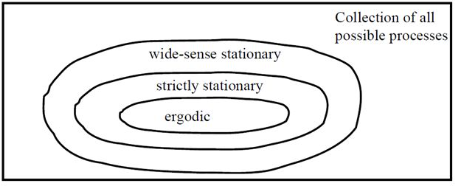
\includegraphics[width=\textwidth]{image.png}
             \caption{Strict Stationary, not depends on time but on difference $\tau$} 
        \end{minipage} \newline \newline
\begin{itemize}
\item  Expectation: 
$$ \mu_X(t) = \mathbb{E}[X(t,A)] = \sum_A X(t,A)f_A(a) $$
$$ \mu_X(t) = \mathbb{E}[X(t,A)] = \int_A X(t,A)f_A(a)\,dA $$

\item Auto-correlation function:
$$ R_{XX}(t,t+\tau) = \mathbb{E}[X(t)X(t+\tau)] $$

\item Auto-covariance function:
\begin{align*}
 \text{Cov}_{XX}(t,t+\tau) &= R_{XX}(t,t+\tau) - \mu_{X}(t) \mu_{X}(t+\tau)\\
 &=\mathbb{E}[X(t)X(t+\tau)]    -\mathbb{E}[X(t)] \mathbb{E}[X(t+\tau)] 
\end{align*}

\item Auto-correlation Coefficient Function:
$$
\rho_{X X}(t, t+\tau)=\frac{\operatorname{Cov}_{X X}(t, t+\tau)}{\sigma_X(t) \sigma_X(t+\tau)}
$$

\item Wide Sense Stationary Process WSSP:
$$\text{Expectation = Constant, Not depend on time}$$
$$ R_{XX}(t,t+\tau) = \mathbb{E}[X(t)X(t+\tau)]= R_{XX}(\tau)$$
$$\text{ depend on time difference only}$$



\item Average power for WSSP:
$$ R_{XX}(\tau = 0) = \mathbb{E}[X(t)X(t+0)] = \mathbb{E}[X^2(t)]  $$
\item Properties of WSSP: \\
\begin{itemize}
    \item Power Spectral Density $S_{X X}(f)=\mathcal{F}\left\{R_{X X}(\tau)\right\}$
    \item Average Power $=R_{X X}(0)=\int_{-\infty}^{\infty} S_{XX}(f) df$
    \item $R_{XX}(\tau)=R_{X X}(-\tau)$ (Even function)
    \item $R_{X X}(\tau)$ is maximum at the origin.
\end{itemize}
\item Properties of Strict Stationary Process SSP:
\begin{itemize}
    \item  $\mu_X=0$
    \item  $R_{X X}(t, t+\tau) =R_{X X}(\tau) $
    \item  $\rho_{X X}(t, t+\tau)=\frac{\operatorname{Cov}_{X X}(\tau)}{\operatorname{Cov}_{X X}(0)}$
    \item $\operatorname{Cov}_{X X}(\tau) = R_{X X}(\tau) - \mu_X^2$
    \item {IID} = Independent Identical distributions
\end{itemize}
\item Properties of White Noise:
\begin{itemize}
    \item  $R_{X X}(\tau)=N_0 \delta(\tau)$
    \item  $ S_{X X}(f)=N_0 $
    \item For the zero-mean signals $N_0=\sigma_X^2$
\end{itemize}

\item Cross-Correlation Function:
\begin{itemize}
    \item $R_{X Y}(t, t+\tau)=E(X(t) Y(t+\tau))$
    \item $R_{X Y}(t, t+\tau) \neq R_{Y X}(t, t+\tau)$
\item If $R_{X Y}(t, t+\tau)=0$ the $X$ and $Y$ are orthogonal.
\item If $X$ and $Y$ are independent, then $R_{X Y}(t, t+\tau)= C$
\end{itemize}

\item Cross-Covariance Function:

\begin{itemize}
    \item $
\operatorname{Cov}_{X Y}(t, t+\tau)=R_{X Y}(t, t+\tau)-\mu_X(t) \mu_Y(t+\tau)
$
\item If $\operatorname{Cov}_{X Y}(t, t+\tau)=0$ the $X$ and $Y$ are Uncorrelated.
\end{itemize}

\item The time-averaged mean:
$$
\langle X(t)\rangle=\lim _{T \rightarrow \infty} \frac{1}{2 T} \int_{-T}^T X(t) dt
$$

\item The time-averaged auto-correlation function:
$$
\langle X(t) X(t+\tau)\rangle=\lim _{T \rightarrow \infty} \frac{1}{2 T} \int_{-T}^T X(t) X(t+\tau) dt
$$

\item The WSS Signal is Called "Ergodic in its mean" if:
$$
E(X(t))=\langle X(t)\rangle
$$

\item  The WSS Signal is Called "Ergodic in its auto-correlation function" if:
$$
R_{X X}(\tau)=\langle X(t) X(t+\tau)\rangle
$$ 
\end{itemize}

\end{multicols*}

\section{Fast-View: Table of Distributions} 


\begin{center}
\renewcommand{\arraystretch}{3.7}
\begin{tabular}{cccccc}
\textbf{Distribution} & \textbf{PMF/PDF and Support} & \textbf{Expected Value}  & \textbf{Variance} & \textbf{MGF}\\
\hline 
\shortstack{Bernoulli \\ \Bern($p$)} & \shortstack{$P(X=1) = p$ \\$ P(X=0) = q=1-p$} & $p$ & $pq$ & $q + pe^t$ \\
\hline
\shortstack{Binomial \\ \Bin($n, p$)} & \shortstack{$P(X=k) = {n \choose k}p^k q^{n-k}$  \\ $k \in \{0, 1, 2, \dots n\}$}& $np$ & $npq$ & $(q + pe^t)^n$ \\
\hline
\shortstack{Geometric \\ \Geo($p$)} & \shortstack{$P(X=k) = q^{k-1}p$  \\ $k \in \{$1, 2, \dots $\}$}& $1/p$ & $q/p^2$ & $\frac{pe^t}{1-qe^t}, \, qe^t < 1$\\
\hline
\hline
\shortstack{Poisson \\ \Pois($\lambda$)} & \shortstack{$P(X=k) = \frac{e^{-\lambda}\lambda^k}{k!}$ \\ $k \in \{$0, 1, 2, \dots $\}$} & $\lambda$ & $\lambda$ & $e^{\lambda(e^t-1)}$ \\
\hline
\hline
\shortstack{Uniform \\ \Unif($a, b$)} & \shortstack{$ f(x) = \frac{1}{b-a}$ \\$ x \in (a, b) $} & $\frac{a+b}{2}$ & $\frac{(b-a)^2}{12}$ &  $\frac{e^{tb}-e^{ta}}{t(b-a)}$\\
\hline
\shortstack{Normal \\ $\N(\mu, \sigma^2)$} & \shortstack{$f(x) = \frac{1}{\sigma \sqrt{2\pi}} e^{-\sfrac{(x - \mu)^2}{(2 \sigma^2)}}$ \\ $x \in (-\infty, \infty)$} & $\mu$  & $\sigma^2$ & $e^{t\mu + \frac{\sigma^2t^2}{2}}$\\
\hline
\shortstack{Exponential \\ $\Expo(\lambda)$} & \shortstack{$f(x) = \lambda e^{-\lambda x}$\\$ x \in (0, \infty)$} & $\frac{1}{\lambda}$  & $\frac{1}{\lambda^2}$ & $\frac{\lambda}{\lambda - t}, \, t < \lambda$\\
\hline
\shortstack{Erlang-k \\ $\text{Erlang}(\lambda, k)$} & \shortstack{$f(x) = \frac{\lambda^x x^{k-1} e^{-\lambda x}}{(k-1)!}$\\$ x \in (0, \infty)$} & $\frac{k}{\lambda}$  & $\frac{k}{\lambda^2}$ & $\left(\frac{\lambda}{\lambda + t} \right)^k, \, t < \lambda$\\
\hline
\shortstack{Gamma \\ $\Gam(a, \lambda)$} & \shortstack{$f(x) = \frac{1}{\Gamma(a)}(\lambda x)^ae^{-\lambda x}\frac{1}{x}$\\$ x \in (0, \infty)$} & $\frac{a}{\lambda}$  & $\frac{a}{\lambda^2}$ & $\left(\frac{\lambda}{\lambda - t}\right)^a, \, t < \lambda$\\
\hline
\shortstack{Chi-Square \\ $\chi_n^2$} & \shortstack{$\frac{1}{2^{n/2}\Gamma(n/2)}x^{n/2 - 1}e^{-x/2}$\\$x \in (0, \infty) $} & $n$  & $2n$ & $(1 - 2t)^{-n/2}, \, t < 1/2$\\
\hline
\shortstack{Rayleigh \\ $\text{R}(r)$} & \shortstack{$\frac{r}{\sigma^2} e^{-r^2 / 2 \sigma^2}$\\$r \in (0, \infty) $} & $\sqrt{\frac{\pi}{2}} \sigma \quad$  & $\quad V(R)= \frac{4-\pi}{2} \sigma^2$ & -\\
\hline
\end{tabular}
\end{center}


\end{document}